% !Mode:: "TeX:UTF-8"

\documentclass[openany,twoside,nofonts,AutoFakeBold,UTF8]{ctexbook}
\usepackage{blindtext}
\usepackage{scrextend}
\usepackage{nomencl}
\usepackage{blkarray}
\usepackage{makecell}
\usepackage{wrapfig}
\usepackage{bbm}
\usepackage{amsmath}
% \addtokomafont{labelinglabel}{\sffamily}
\renewcommand{\footnotesize}{\fontsize{9pt}{10pt}\selectfont}
\def\bd{\boldsymbol}        % 加粗(向量) boldsymbol
\def\e{\mathrm{e}}          % Euler's number
\def\add{\vspace{1ex}}      % 增加行间距
\def\del{\vspace{-1.5ex}}   % 减少行间距
\DeclareMathOperator*{\argmax}{arg\,max}  % 定义取最大值的参数 \argmax_{}
\newcommand\myemptypage{    % 增加空白页
  \null
  \thispagestyle{empty}
  \addtocounter{page}{-1}
  \newpage
}

% !Mode:: "TeX:UTF-8"

\usepackage[a4paper,top=21.5mm,bottom=19.5mm,left=26mm,right=26mm,includehead,includefoot]{geometry}					% 控制页面尺寸
\usepackage{titletoc}       % 控制目录的宏包
\usepackage{titlesec}       % 控制标题的宏包
\usepackage{fancyhdr}       % 页眉和页脚的相关定义
\usepackage{color}          % 支持彩色
\usepackage{graphicx}		% 处理图片
\usepackage{tabularx}		% 可伸缩表格
\usepackage{multirow}       % 表格可以合并多个row
\usepackage{booktabs}       % 表格横的粗线;\specialrule{1pt}{0pt}{0pt}
\usepackage{longtable}      % 支持跨页的表格。
\usepackage{enumitem}       % 使用enumitem宏包,改变列表项的格式
\usepackage{amsmath}        % 公式宏包
\usepackage{amssymb}		% 符号宏包
\usepackage{bm}				% 处理数学公式中的黑斜体的宏包
\usepackage{lmodern}		% 数学公式字体
\usepackage[amsmath,thmmarks,hyperref]{ntheorem}	% 定理类环境宏包
\usepackage[hang]{subfigure}						% 图形或表格并排排列
\usepackage[subfigure]{ccaption}					% 支持双语标题
\usepackage[sort&compress,numbers]{natbib}			% 支持引用缩写的宏包
\usepackage{fontspec}		% 字体设置宏包
%\usepackage{etoolbox}		% primarily towards LaTeX class and package authors.
%\usepackage{xltxtra}		% 提供了针对XeTeX的改进,自动调用xunicode宏包

% 生成有书签的 pdf 及其开关, 该宏包应放在所有宏包的最后, 宏包之间有冲突
\usepackage[xetex,
            bookmarksnumbered=true,
            bookmarksopen=true,
            colorlinks=false,
            pdfborder={0 0 1},
            citecolor=blue,
            linkcolor=red,
            anchorcolor=green,
            urlcolor=blue,
            breaklinks=true
            ]{hyperref}

% 算法的宏包,注意宏包兼容性,先后顺序为float、hyperref、algorithm(2e),否则无法生成算法列表
\usepackage[plainruled,linesnumbered,algochapter]{algorithm2e}
% \usepackage[linesnumbered,ruled,vlined]{algorithm2e}
\SetKwInput{KwIn}{输入}  %<---细节与重点
\SetKwInput{KwOut}{输出}  %<---细节与重点

% \usepackage{listings}		% 为了避免与页眉的兼容问题可将listings放入table环境中
% \definecolor{codegreen}{rgb}{0,0.6,0}
% \definecolor{codepurple}{rgb}{0.58,0,0.82}
% \lstset{%
% 	language={[ISO]C++},				% 设置语言
% 	alsolanguage=Matlab,				% 可以添加多个语言选项
% 	alsolanguage=Verilog,
% 	morekeywords={numerictype,fimath,fipref,fi,trh},
% 	commentstyle=\color{codegreen},		% 注释颜色
% 	keywordstyle=\color{blue},			% 代码关键字颜色
% 	stringstyle=\color{codepurple},		% 代码中字符串颜色
% 	frame=single,			% 设置边框, 
% 	xleftmargin=1.7em,		% 设定listing左边空白 
% 	numbers=left,			% 左侧显示行号
% 	numberstyle=\small,		% 行号字体用小号
% 	breaklines=true,		% 对过长的代码自动换行 
% 	columns=flexible,		% 调整字符之间的距离
% 	tabsize=4				% table 长度
% }
%%%% 设置代码块 %%%%
% 在vscode中使用minted需要先配置python解释器, Ctrl+Shift+P, 输入Python: Select Interpreter选择安装了Pygments的Python版本. 再在setting.json中xelatex和pdflatex的参数中加入 "--shell-escape", 即可
% TeXworks中配置方法参考: https://blog.csdn.net/RobertChenGuangzhi/article/details/108140093
\usepackage{minted}
\renewcommand{\theFancyVerbLine}{
    \sffamily\textcolor[rgb]{0.5,0.5,0.5}{\scriptsize\arabic{FancyVerbLine}}} % 修改代码前序号大小
% 加入不同语言的代码块
\newmintinline{cpp}{fontsize=\small, linenos, breaklines, frame=lines}
\newminted{cpp}{fontsize=\small, baselinestretch=1, linenos, breaklines, frame=lines}
\newmintedfile{cpp}{fontsize=\small, baselinestretch=1, linenos, breaklines, frame=lines}
\newmintinline{matlab}{fontsize=\small, linenos, breaklines, frame=lines}
\newminted{matlab}{fontsize=\small, baselinestretch=1, mathescape, linenos, breaklines, frame=lines}
\newmintedfile{matlab}{fontsize=\small, baselinestretch=1, linenos, breaklines, frame=lines}
\newmintinline{python}{fontsize=\small, linenos, breaklines, frame=lines, python3}  % 使用\pythoninline{代码}
\newminted{python}{fontsize=\small, baselinestretch=1, linenos, breaklines, frame=lines, python3}  % 使用\begin{pythoncode}代码\end{pythoncode}
\newmintedfile{python}{fontsize=\small, baselinestretch=1, linenos, breaklines, frame=lines, python3}  % 使用\pythonfile{代码地址}

% 带圆圈的脚注
\usepackage{pifont}
\usepackage[flushmargin,para,symbol*]{footmisc}
\DefineFNsymbols{circled}{{\ding{192}}{\ding{193}}{\ding{194}}
	{\ding{195}}{\ding{196}}{\ding{197}}{\ding{198}}{\ding{199}}{\ding{200}}{\ding{201}}}
\setfnsymbol{circled}

% 字体设置,Windows自带黑体(simhei.ttf)和宋体(simsun.ttf)
\defaultfontfeatures{Mapping=tex-text}
\setmainfont{Times New Roman}
% \setsansfont{Arial}
\setCJKmainfont{SimSun}
\setCJKsansfont{SimHei}
\setCJKfamilyfont{hei}{SimHei}
\newcommand{\hei}{\CJKfamily{hei}}

% 外文文献pdf插入
\usepackage{pdfpages}

% 符号表
\graphicspath{{figures/}}

%===================================== Cover and TOC =====================================
\begin{document}
% !Mode:: "TeX:UTF-8" 

% 备注
\long\def\zhao#1{\textcolor{red}{\bf **#1**}}

%========================================= Font ==========================================
% 定义字号
\newcommand{\yihao}{\fontsize{26pt}{26pt}\selectfont}       % 一号, 1.倍行距
\newcommand{\xiaoyi}{\fontsize{24pt}{24pt}\selectfont}      % 小一, 1.倍行距
\newcommand{\erhao}{\fontsize{22pt}{22pt}\selectfont}		% 二号, 1.倍行距
\newcommand{\xiaoer}{\fontsize{18pt}{18pt}\selectfont}      % 小二, 单倍行距
\newcommand{\sanhao}{\fontsize{16pt}{16pt}\selectfont}      % 三号, 1.倍行距
\newcommand{\xiaosan}{\fontsize{15pt}{15pt}\selectfont}     % 小三, 1.倍行距
\newcommand{\sihao}{\fontsize{14pt}{14pt}\selectfont}       % 四号, 1.倍行距
\newcommand{\xiaosi}{\fontsize{12pt}{12pt}\selectfont}      % 小四, 1.倍行距
\newcommand{\wuhao}{\fontsize{10.5pt}{10.5pt}\selectfont}   % 五号, 单倍行距
\newcommand{\xiaowu}{\fontsize{9pt}{9pt}\selectfont}        % 小五, 单倍行距

% 默认字体
\makeatletter
\renewcommand\normalsize{%
	\@setfontsize\normalsize{12pt}{12pt}%
	\setlength\abovedisplayskip{8pt}%
	\setlength\abovedisplayshortskip{8pt}%
	\setlength\belowdisplayskip{\abovedisplayskip}%
	\setlength\belowdisplayshortskip{\abovedisplayshortskip}%
	\let\@listi\@listI%
}

% 设置行距和段落间垂直距离
\setlength{\parindent}{2em}
\setlength{\parskip}{3pt plus1pt minus1pt}
\def\defaultfont{\renewcommand{\baselinestretch}{1.5}\normalsize\selectfont}

% 设置字间距,使每行37个字,若要减少每行字数(一般以34个),将0.56pt的值增加
\renewcommand{\CJKglue}{\hskip 0.56pt plus 0.08\baselineskip}

% 公式跨页设置,公式之前可以换页,公式出现在页面顶部
\predisplaypenalty=0
\allowdisplaybreaks[4]

%========================================= TOC ===========================================
% 中文目录格式定义
\renewcommand\contentsname{目\quad 录}
\titlecontents{chapter}[3.8em]{\hspace{-3.8em}}{\thecontentslabel~~}{}{\titlerule*[4pt]{.}\contentspage}
\dottedcontents{section}[38pt]{}{22pt}{0.3pc}
\dottedcontents{subsection}[70pt]{}{32pt}{0.3pc}

% 英文目录格式定义: 细点\@dottedtocline  粗点\@dottedtoclinebold
\renewcommand*\l@chapter{\@dottedtocline{0}{0em}{5em}}
\renewcommand*\l@section{\@dottedtocline{1}{1em}{1.8em}}
\renewcommand*\l@subsection{\@dottedtocline{2}{2.9em}{2.5em}}
\def\@dotsep{0.75}           % 定义英文目录的点间距
\setlength\leftmargini {50pt}
\setlength\leftmarginii {50pt}
\def\engcontentsname{CONTENTS}
\newcommand\tableofengcontents{
	\@restonecolfalse
	\chapter*{\engcontentsname  %chapter*上移一行,避免在toc中出现。
		\@mkboth{%
			\engcontentsname}{\engcontentsname}}
	\@starttoc{toe}%
	\if@restonecol\twocolumn\fi
}

%======================================= Chapter =========================================
% 章节格式定义
\CTEXsetup[number={\arabic{chapter}}]{chapter}
\renewcommand\chaptername{\thechapter}
\CTEXsetup[name={,}]{chapter}
\setcounter{secnumdepth}{4} \setcounter{tocdepth}{2}
\titleformat{\chapter}{\center\sanhao}{\chaptertitlename}{0.5em}{}
\titlespacing{\chapter}{0pt}{-5mm}{5mm}
\titleformat{\section}{\xiaosan}{\thesection}{0.5em}{}
\titlespacing{\section}{0pt}{3mm}{3mm}
\titleformat{\subsection}{\sihao}{\thesubsection}{0.5em}{}
\titlespacing{\subsection}{2.13em}{3mm}{3mm}

% 重新定义BiChapter命令,可实现标题手动换行,但不影响目录
\def\BiChapter{\relax\@ifnextchar [{\@BiChapter}{\@@BiChapter}}
\def\@BiChapter[#1]#2#3{\chapter[#1]{#2}
    \addcontentsline{toe}{chapter}{\xiaosi \thechapter\hspace{0.5em} #3}}
\def\@@BiChapter#1#2{\chapter{#1}
    \addcontentsline{toe}{chapter}{\xiaosi \thechapter\hspace{0.5em}{\boldmath #2}}}
% 定义双标题
\newcommand{\BiSection}[2]{
	\section{#1}
	\addcontentsline{toe}{section}{\protect\numberline{\csname thesection\endcsname}#2}
}
\newcommand{\BiSubsection}[2]{
	\subsection{#1}
	\addcontentsline{toe}{subsection}{\protect\numberline{\csname thesubsection\endcsname}#2}
}
\newcommand{\BiSubsubsection}[2]{
    \subsubsection{#1}
    \addcontentsline{toe}{subsubsection}{\protect\numberline{\csname thesubsubsection\endcsname}#2}
}

% 该附录命令适用于有章节的完整附录和用于发表文章和简历的附录
\newcommand{\BiAppChapter}[2]{
	\phantomsection 
	\chapter{#1}
	\addcontentsline{toe}{chapter}{\xiaosi Appendix \thechapter~~#2}
}
\newcommand{\BiAppendixChapter}[2]{
	\phantomsection
	\markboth{#1}{#1}
	\addcontentsline{toc}{chapter}{\xiaosi #1}
	\addcontentsline{toe}{chapter}{\xiaosi #2}  \chapter*{#1}
}
\newcommand{\Abstract}[2]{
	\phantomsection
	\markboth{#1}{#1}
	\chapter*{#1}
}


%======================================== Header =========================================
% 定义页眉和页脚
\newcommand{\makeheadrule}{
\rule[8pt]{\textwidth}{0.4pt} \\[-22pt]
\rule{\textwidth}{0.4pt}}
\renewcommand{\headrule}{
    {\if@fancyplain\let\headrulewidth\plainheadrulewidth\fi
     \makeheadrule}}
\pagestyle{fancyplain}

% 不要注销这一行,否则页眉会变成:“第1章1  绪论”样式
\renewcommand{\chaptermark}[1]{\markboth{\chaptertitlename~\ #1}{}}
\fancyhf{}
\fancyhead[CO]{\wuhao\leftmark}
\fancyhead[CE]{\wuhao 西安交通大学本科毕业设计(论文)}%
\fancyfoot[LE,RO]{\wuhao\thepage}

%======================================= Theorem =========================================
% 定理环境格式定义
\theoremstyle{plain}
\theorembodyfont{\rmfamily}
\theoremheaderfont{\hei\rmfamily}
\setlength{\theorempreskipamount}{8pt}
\setlength{\theorempostskipamount}{8pt}
\theoremseparator{:}
\theoremsymbol{$\Diamond$} \newtheorem{definition}{\hskip 2em \hei 定义}[chapter]
\theoremsymbol{$\blacklozenge$} \newtheorem{example}{\hskip 2em \hei 例}[chapter]
\theoremsymbol{$\square$} \newtheorem{theorem}{\hskip 2em \hei 定理}[chapter]
\theoremsymbol{$\blacksquare$} \newtheorem*{proof}{\hskip 2em \hei 证明}

%========================================= FTE ===========================================
% 图表公式的编号为1-1格式,子图编号为 a) 的格式
\renewcommand{\thefigure}{\arabic{chapter}-\arabic{figure}}
\renewcommand{\thesubfigure}{(\alph{subfigure})}
\renewcommand{\p@subfigure}{\thefigure~}
\renewcommand{\thetable}{\arabic{chapter}-\arabic{table}}%使表编号为 7-1 的格式
\renewcommand{\theequation}{\arabic{chapter}-\arabic{equation}}%使公式编号为 7-1 的格式

% 定制浮动图形和表格标题样式
\captionnamefont{\wuhao}
\captiontitlefont{\wuhao}
\captiondelim{~~}
\hangcaption
\renewcommand{\subcapsize}{\wuhao}
% \setlength{\abovecaptionskip}{0pt}
\setlength{\abovecaptionskip}{-4ex}  % 由于minted会增大图像与标题间距需要进行缩小
\setlength{\belowcaptionskip}{0pt}

% 关于公式的几个定义
\renewcommand{\Re}{\mathrm{Re}}
\renewcommand{\Im}{\mathrm{Im}}
\newcommand{\mbf}[1]{\mathbf{#1}}
\newcommand{\Exp}{\mathrm{E}}
\newcommand{\dif}{\mathrm{d}}
\newcommand{\seq}[2]{#1_1,#1_2,\cdots,#1_#2}
\newcommand{\iprod}[2]{\langle #1,#2 \rangle}

% 调整罗列环境的布局
\setitemize{leftmargin=3.23em,itemsep=0em,partopsep=0em,parsep=0em,topsep=-0em}
% \setenumerate{leftmargin=3.45em,itemsep=0em,partopsep=0em,parsep=0em,topsep=0em}
\setenumerate{leftmargin=2em,itemsep=0em,partopsep=0em,parsep=0em,topsep=0em}

% 自定义项目列表标签及格式 \begin{publist} 列表项 \end{publist}
\newcounter{pubctr} %自定义新计数器
\newenvironment{publist}{
	\begin{list}{[\arabic{pubctr}]}{
     \usecounter{pubctr}
     \setlength{\leftmargin}{2em}     % 左边界
     \setlength{\labelsep}{1em}       % 标号和列表项之间的距离,默认0.5em
     \setlength{\parsep}{0ex}         % 段落间距
     \setlength{\itemsep}{0ex}        % 标签间距
    }}
{\end{list}}%

% 更改算法标题
\renewcommand{\algorithmcfname}{算法}
\renewcommand{\algocf@captiontext}[2]{\wuhao#1\algocf@typo ~ \AlCapFnt{}#2}
\renewcommand\thealgocf{\csname the\algocf@within\endcsname-\@arabic\c@algocf}
\SetAlCapSty{textrm}
\SetAlCapSkip{1ex}

% 更改代码标题
% \renewcommand{\lstlistingname}{代码}
% \renewcommand{\thelstlisting}{\arabic{chapter}-\arabic{lstlisting}}

%======================================== Other ==========================================
% 避免宏包 hyperref 和 arydshln 不兼容带来的目录链接失效的问题。
\def\temp{\relax}
\let\temp\addcontentsline
\gdef\addcontentsline{\phantomsection\temp}
\gdef\hitempty{}

\renewcommand\frontmatter{\cleardoublepage
	\@mainmatterfalse
	\pagenumbering{Roman}
}

% 引用改为上标
\newcommand{\upcite}[1]{\textsuperscript{\cite{#1}}}

\makeatother


%======================================= Main Body =======================================
\mainmatter\defaultfont\sloppy\raggedbottom

%======================================= Reference =======================================

%======================================= Appendix ========================================
% !Mode:: "TeX:UTF-8" 

\appendix
\defaultfont
\renewcommand{\appendixname}{附录~\Alph{chapter}}
\CTEXsetup[name={附录}]{chapter}

\renewcommand{\thefigure}{\Alph{chapter}-\arabic{figure}}
\renewcommand{\thetable}{\Alph{chapter}-\arabic{table}}
\renewcommand{\theequation}{附录\Alph{chapter}-\arabic{equation}}
% \renewcommand{\thelstlisting}{\Alph{chapter}-\arabic{lstlisting}}

% \setlength{\abovecaptionskip}{0ex}  % 由于minted会增大图像与标题间距需要进行缩小  % 附录配置

\BiAppChapter{外文文献原文}{Translation}

\setcounter{page}{36}
{\centering
\vspace{-5ex}
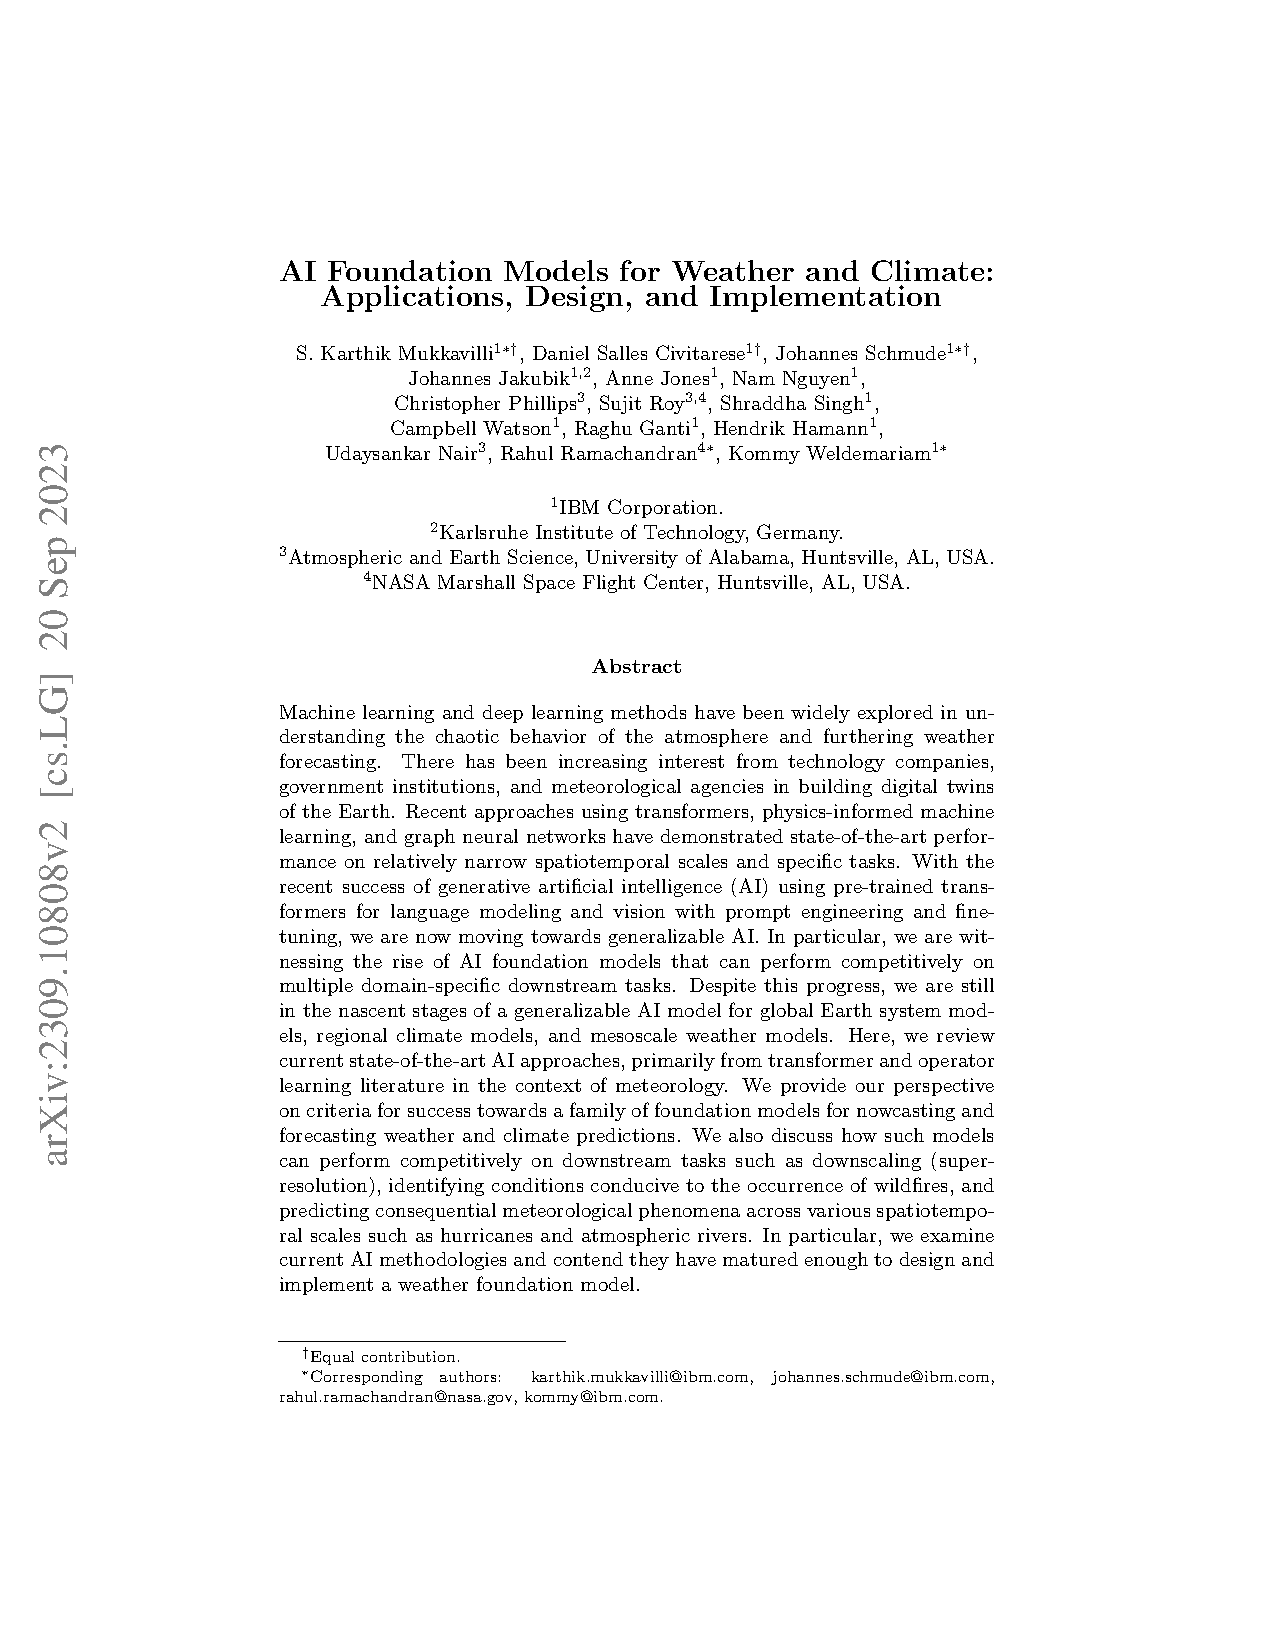
\includegraphics[width=\textwidth, page=1, trim = 15mm 20mm 15mm 20mm]{pdfs/师梓豪_2204112376_外文翻译原文.pdf}
\includegraphics[width=\textwidth, page=2, trim = 25mm 20mm 25mm 20mm]{pdfs/师梓豪_2204112376_外文翻译原文.pdf}
\includegraphics[width=\textwidth, page=3, trim = 25mm 20mm 25mm 20mm]{pdfs/师梓豪_2204112376_外文翻译原文.pdf}
\includegraphics[width=\textwidth, page=4, trim = 25mm 20mm 25mm 20mm]{pdfs/师梓豪_2204112376_外文翻译原文.pdf}
\includegraphics[width=\textwidth, page=5, trim = 25mm 20mm 25mm 20mm]{pdfs/师梓豪_2204112376_外文翻译原文.pdf}
\includegraphics[width=\textwidth, page=6, trim = 25mm 20mm 25mm 20mm]{pdfs/师梓豪_2204112376_外文翻译原文.pdf}
\includegraphics[width=\textwidth, page=7, trim = 25mm 20mm 25mm 20mm]{pdfs/师梓豪_2204112376_外文翻译原文.pdf}
\includegraphics[width=\textwidth, page=8, trim = 25mm 20mm 25mm 20mm]{pdfs/师梓豪_2204112376_外文翻译原文.pdf}
\includegraphics[width=\textwidth, page=9, trim = 25mm 20mm 25mm 20mm]{pdfs/师梓豪_2204112376_外文翻译原文.pdf}
\includegraphics[width=\textwidth, page=10, trim = 25mm 20mm 25mm 20mm]{pdfs/师梓豪_2204112376_外文翻译原文.pdf}
\includegraphics[width=\textwidth, page=11, trim = 25mm 20mm 25mm 20mm]{pdfs/师梓豪_2204112376_外文翻译原文.pdf}
\includegraphics[width=\textwidth, page=12, trim = 25mm 20mm 25mm 20mm]{pdfs/师梓豪_2204112376_外文翻译原文.pdf}
\includegraphics[width=\textwidth, page=13, trim = 25mm 20mm 25mm 20mm]{pdfs/师梓豪_2204112376_外文翻译原文.pdf}
\includegraphics[width=\textwidth, page=14, trim = 25mm 20mm 25mm 20mm]{pdfs/师梓豪_2204112376_外文翻译原文.pdf}
\includegraphics[width=\textwidth, page=15, trim = 25mm 20mm 25mm 20mm]{pdfs/师梓豪_2204112376_外文翻译原文.pdf}
\includegraphics[width=\textwidth, page=16, trim = 25mm 20mm 25mm 20mm]{pdfs/师梓豪_2204112376_外文翻译原文.pdf}
}
% 外文文献以图片的形式插入,不会发生失真  % 外文原文

\BiAppChapter{外文文献译文}{Translation}

{\centering
\vspace{-5ex}
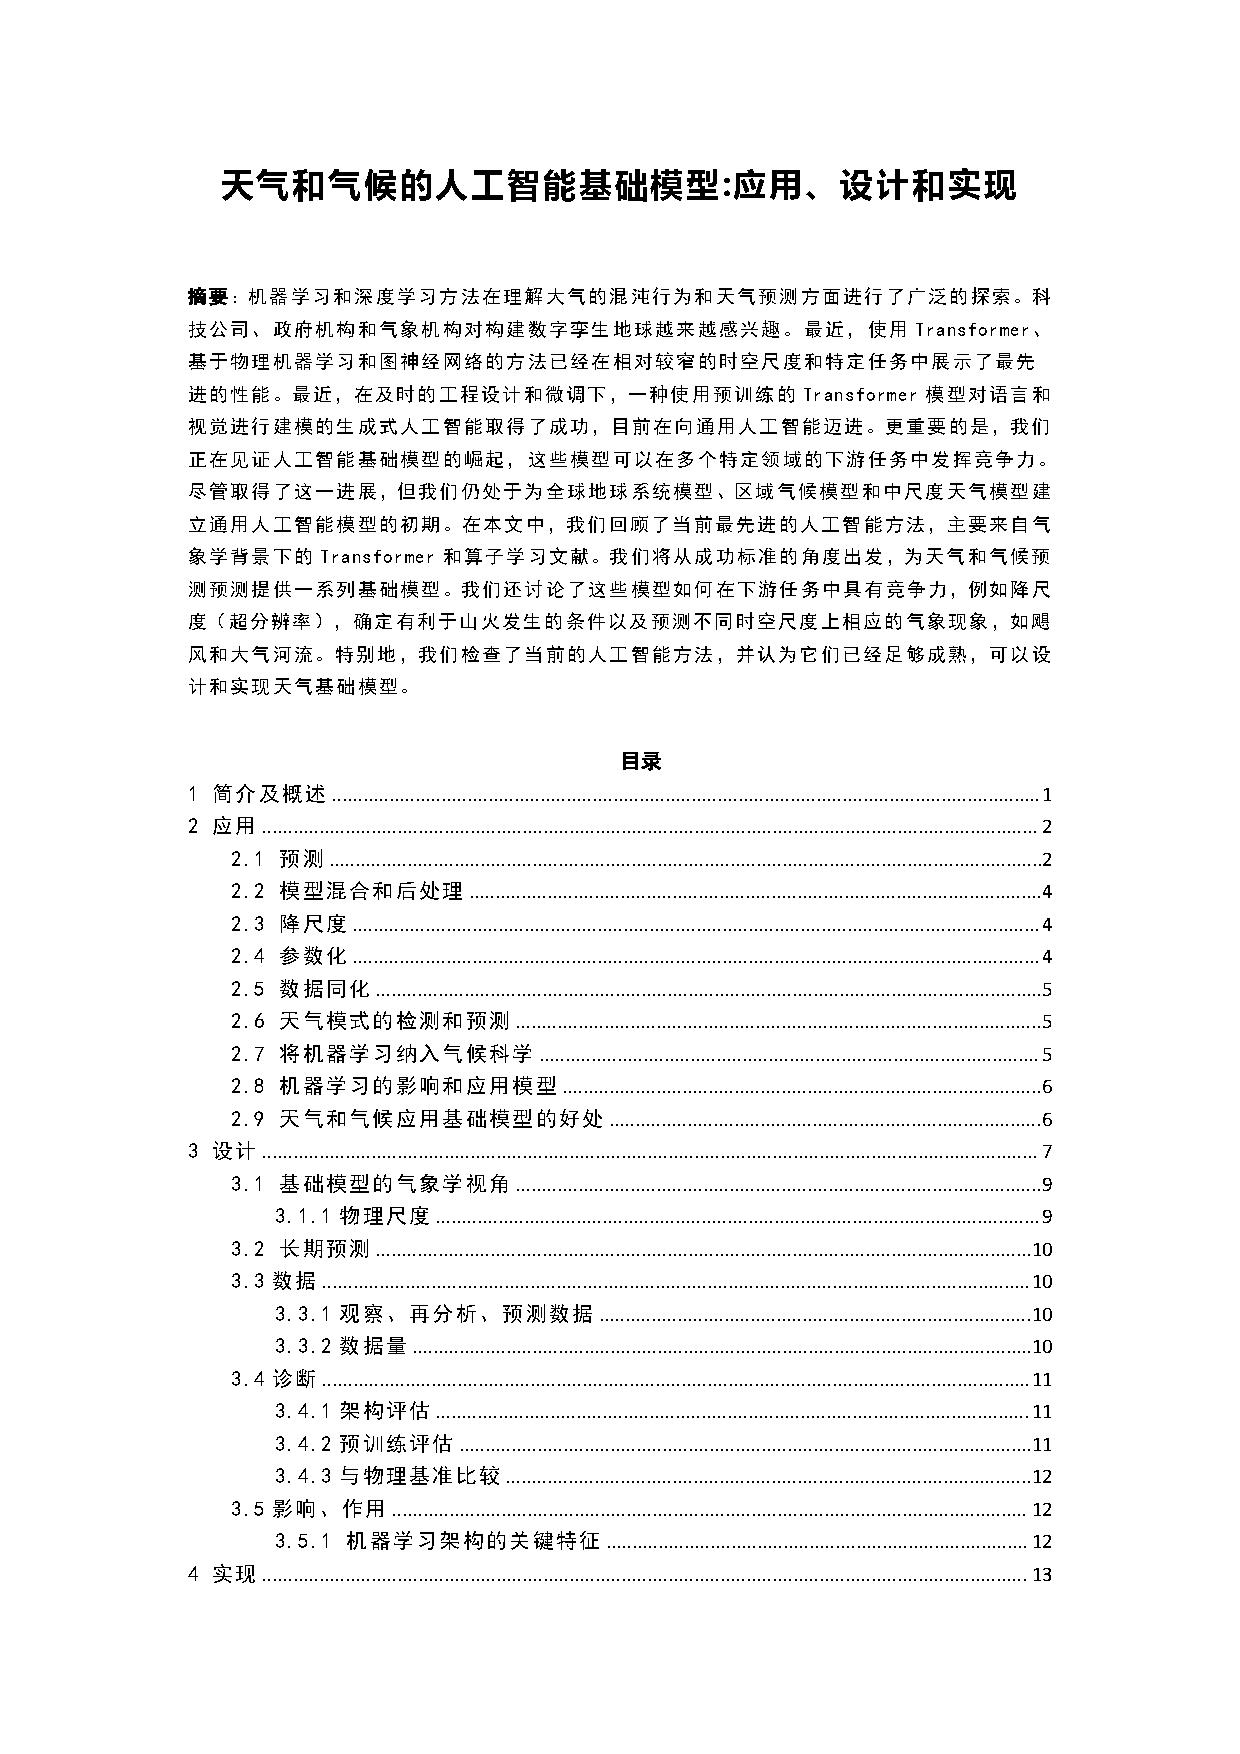
\includegraphics[width=\textwidth, page=1, trim = 15mm 20mm 15mm 20mm]{pdfs/师梓豪_2204112376_外文翻译译文.pdf}
\includegraphics[width=\textwidth, page=2, trim = 15mm 20mm 15mm 20mm]{pdfs/师梓豪_2204112376_外文翻译译文.pdf}
\includegraphics[width=\textwidth, page=3, trim = 15mm 20mm 15mm 20mm]{pdfs/师梓豪_2204112376_外文翻译译文.pdf}
\includegraphics[width=\textwidth, page=4, trim = 15mm 20mm 15mm 20mm]{pdfs/师梓豪_2204112376_外文翻译译文.pdf}
\includegraphics[width=\textwidth, page=5, trim = 15mm 20mm 15mm 20mm]{pdfs/师梓豪_2204112376_外文翻译译文.pdf}
\includegraphics[width=\textwidth, page=6, trim = 15mm 20mm 15mm 20mm]{pdfs/师梓豪_2204112376_外文翻译译文.pdf}
\includegraphics[width=\textwidth, page=7, trim = 15mm 20mm 15mm 20mm]{pdfs/师梓豪_2204112376_外文翻译译文.pdf}
\includegraphics[width=\textwidth, page=8, trim = 15mm 20mm 15mm 20mm]{pdfs/师梓豪_2204112376_外文翻译译文.pdf}
\includegraphics[width=\textwidth, page=9, trim = 15mm 20mm 15mm 20mm]{pdfs/师梓豪_2204112376_外文翻译译文.pdf}
\includegraphics[width=\textwidth, page=10, trim = 15mm 20mm 15mm 20mm]{pdfs/师梓豪_2204112376_外文翻译译文.pdf}
}

% 外文文献以图片的形式插入,不会发生失真  % 外文翻译

\end{document} 
